\documentclass[../TDON2_inter.tex]{subfiles}%

\begin{document}
\section[s]"1"{Interférences de 2 ondes sonores frontales}

\enonce{%
	\noindent
	\begin{minipage}{0.65\linewidth}
		Dans le montage ci-contre, les deux haut-parleurs, notés HP1 et HP2 et
		séparés de la distance $2D$, sont alimentés en parallèle par une même
		tension électrique~: les deux sources sonores émettent donc des vibrations
		$p_1(t)$ et $p_2(t)$ de même pulsation $\w$, même phase à l'origine $\f_0$
		et même amplitude $P_0$. Les deux ondes arrivent au point M d'abscisse $x$
		avec des phases différentes et donc interfèrent.
	\end{minipage}
	\hfill
	\begin{minipage}{0.35\linewidth}
		\begin{center}
			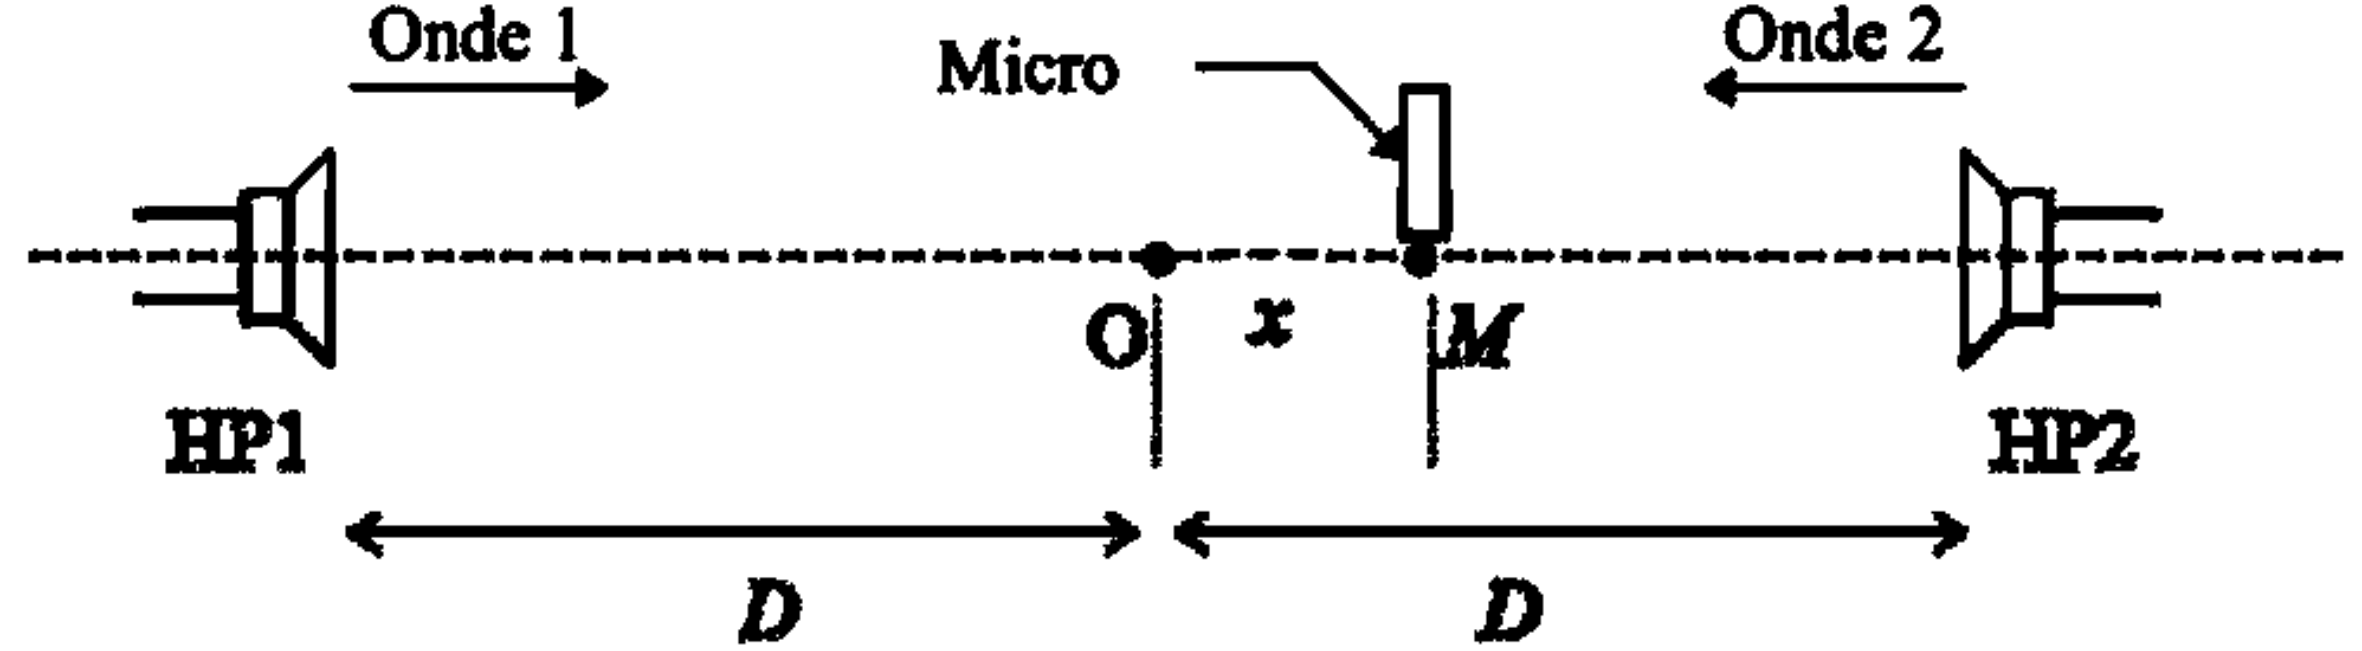
\includegraphics[width=\linewidth]{ondes_front-plain}
		\end{center}
	\end{minipage}
	\smallbreak
	On considère que les ondes sonores se propagent sans déformation ni
	atténuation à la célérité $c$ constante.
}

\QR{%
	Exprimer le déphasage $\D\f$ au point M entre les ondes issues de HP1
	et HP2.
}{%
	À partir de HP1, les ondes parcourent la distance $D+x$ pour arriver
	au micro. À partir de HP2, elles parcourent la distance $D-x$. Ainsi,
	\begin{align*}
		\D\f_{1/2}(\Mr)
		 & = -k\D L_{1/2}(\Mr) + \underbrace{\D\f_0(\Mr)}_
		{\mathclap{= 0 \text{ d'après l'énoncé}}}
		\\
		 & = - k \left( {\rm \abs{HP_1M} - \abs{HP_2M}} \right)
		\\
		 & = - k \left( \cancel{D}+x - (\cancel{D}-x) \right)
		\\
		\Lra
		\Aboxed{%
			\D\f_{1/2}(\Mr)
		 & = - 2kx}
	\end{align*}
}

\QR{%
	En déduire l'amplitude de l'onde sonore résultante au point M.
}{%
	Les ondes $p_1(t)$ et $p_2(t)$ étant de même amplitude $P_0$, on a que
	l'onde somme $p(t) = p_1(t) + p_2(t)$ est d'amplitude $P(\Mr)$ telle que
	\[
		P(\Mr) = 2P_0\cos(\frac{\D\f(\Mr)}{2})
		\Lra
		\boxed{P = 2P_0\cos(-kx)}
	\]
}

\QR{%
	Déterminer les positions $x_n$ pour lesquelles il y a interférences
	constructives au point M.
}{%
	On a interférences constructives si l'amplitude est maximale, ici pour
	$\cos(-kx_n) = \pm 1 \Lra -kx_n = n\pi$. Or,
	\begin{gather*}
		-kx_n = n\pi
		\Lra
		- \frac{2\cancel{\pi}}{\lambda}x_n = n\cancel{\pi}
		\Lra
		\boxed{%
			x_n = n \frac{\lambda}{2}
		}
	\end{gather*}
}

\QR{%
	Exprimer la distance $d$ entre deux maximums successifs d'intensité
	sonore.
}{%
	Les maximums se trouvent aux positions $x_n$. La distance entre deux
	maximums est donc
	\begin{gather*}
		\boxed{d = x_{n+1} - x_n = \frac{\lambda}{2}}
	\end{gather*}
}

\QR{%
	Expérimentalement on trouve $d = \SI{21.2}{cm}$ pour une fréquence
	sonore $f = \SI{800}{Hz}$. En déduire la valeur de la célérité du son
	dans l'air pour cette expérience.
}{%
	Étant donné que $\lambda = cT = c/f$, on trouve
	\begin{gather*}
		\frac{\lambda}{2} = d
		\Lra
		\frac{c}{2f} = d
		\Lra
		\boxed{c = 2df}
		\qavec
		\left\{
		\begin{array}{rcl}
			d & = & \SI{21.2e-2}{m} \\
			f & = & \SI{800}{Hz}
		\end{array}
		\right.\\
		\mathrm{A.N.~:}\quad
		\boxed{c = \SI{339}{m.s^{-1}}}
	\end{gather*}
	C'est la valeur usuelle de célérité du son dans l'air à
	\SI{20}{\degreeCelsius}.
}
\end{document}
